% This is an example of how to format a thesis with LaTeX the
% simplest possible way (permitted beginning in 2010).
% NO UGA STYLE SHEET IS NEEDED.

\documentclass[12pt]{report}
\usepackage{fullpage}
\usepackage{setspace}\doublespacing    % important!
\usepackage{graphicx}
\usepackage{cite}
\usepackage{adjustbox}
\textfloatsep 0.75in                   % important with double spacing

\begin{document}

% Make the official abstract page
\newpage
\thispagestyle{empty}
\vspace*{18pt}
\begin{center}
\textsc{Structure Forming Processes in\\Mesoscopic Polymer Systems}\\[18pt]
by\\[18pt]
\textsc{Tomas Koci}\\[12pt]
(Under the direction of Michael Bachmann)\\[12pt]
\textsc{Abstract}
\end{center}
This is going to be the best abstract ever :)

% Display the index words (this is a bit fancy):
\begin{list}{\sc Index words:\hfill}{\labelwidth 1.2in\leftmargin 1.4in\labelsep 0.2in}
\item 
\begin{flushleft}\singlespacing
Polymer Aggregation,
Monte Carlo Simulations,
Parallel Tempering,
Multicanonical Sampling,
Canonical Analysis, 
Microcanonical Inflection-Point Analysis,
Flexible Polymer,
Structural Transitions,
Finite Systems,
Finite-Size Effects
\end{flushleft}
\end{list}



% Make the official title page
\newpage
\thispagestyle{empty}
\vspace*{18pt}
\begin{center}
\textsc{Structure Forming Processes in\\Mesoscopic Polymer Systems}\\[18pt]
by\\[18pt]
\textsc{Tomas Koci}\\[12pt]
B.A., The Juilliard School, 2008\\
\vfill
A Dissertation Submitted to the Graduate Faculty \\
of The University of Georgia in Partial Fulfillment \\
of the \\
Requirements for the Degree \\[10pt]
\textsc{Doctor of Philosophy}\\[36pt]
\textsc{Athens, Georgia}\\[18pt]
2016
\end{center}

% Make the copyright page
\newpage
\thispagestyle{empty}
\vspace*{5.5in}
\begin{center}
\copyright 2016 \\
Tomas Koci \\
All Rights Reserved
\end{center}

% Make the approval page
\newpage
\thispagestyle{empty}
\vspace*{18pt}
\begin{center}
\textsc{Structure Forming Processes in\\Mesoscopic Polymer Systems}\\[18pt]
by\\[18pt]
\textsc{Tomas Koci}
\end{center}
\vfill
\begin{flushleft}\singlespacing
\hskip 200pt {Approved:}\\
\vskip 12pt
% Two major professors.  If you have only one, change word to "Professor".
\hspace*{200pt}\makebox[100pt][l]{Major Professor:}Michael Bachmann\\
\vskip 12pt
% Committee (use as many lines as needed)
\hspace*{200pt}\makebox[100pt][l]{Committee:       }Steven P. Lewis\\
\hspace*{200pt}\makebox[100pt][l]{~                }Heinz-Bernd Schuttler\\
% Approval words
\vfill
Electronic Version Approved:\\[12pt]
Alan Dorsey\\
Dean of the Graduate School\\
The University of Georgia\\
July 2016
\end{flushleft}


% Now we begin the regular LaTeX document.
% You may want to have a regular LaTeX title page here...

\chapter*{Acknowledgments}
\pagenumbering{roman}
\setcounter{page}{4}

\setcounter{tocdepth}{1}
\tableofcontents
\listoffigures  % if any
\listoftables % if any

\chapter{Introduction}
\pagenumbering{arabic}
\setcounter{page}{1}
Kickass intro...


\chapter{Elements of Statistical Mechanics}
\label{chap:elements_of_stat_mech}
Statistical mechanics aims at explaining the microscopic origins of macroscopic properties of systems with large numbers of degrees of freedom. The exact solution for a single phase space trajectory of a complex system requires enormous computational efforts and in most cases provides only a limited insight. In contrast to the chaotic nature of most phase space trajectories, collective system properties such as entropy, pressure, or temperature, for the most part exhibit relatively simple behavior. The formalism of statistical mechanics allows us to study these properties by considering the average behavior of a large number of identically prepared systems, i.e. the statistical ensemble. It is well established that in the thermodynamic limit all ensembles become equivalent. However this is emphatically not true in the case of intrinsically finite systems for which the choice of an ensemble is non-trivial. Therefore, I shall briefly discuss several prominent statistical ensembles starting with the most fundamental one, the \textit{microcanonical ensemble}.

\section{The microcanonical ensemble}
\label{sec:mic_ensemble}
Let us consider a mechanically and adiabatically isolated system with a constant number of particles $(N)$, volume $(V)$, and energy $(E)$. At any given moment, the system is to be found in a particular microstate $\mu$, which is represented by a point in a $6N$ dimensional phase-space. At a fixed energy $E$, the accessible microstates are constrained to the surface of constant energy $\mathcal{H}(\mu) = E$, where $\mathcal{H}$ is the Hamiltonian of the system. The total number of microstates corresponding to a macrostate with a fixed energy $E$ is obtained by calculating the density of states\footnote{Please refer to section 2.3 for detailed discussion of alternative definitions of the density of states.}
\begin{equation}
\label{eq:densityOfStatesTheoretic}
g(E) = \int \mathcal{DP}\mathcal{DQ} \:\: \delta(E - \mathcal{H}(\mathcal{P},\mathcal{Q})),
\end{equation} 
where 
\begin{equation}
\mathcal{DP}\mathcal{DX} = \prod_{n = 1}^{N} \frac{d^{3}p_{n}d^{3}x_{n}}{(2 \pi \hbar)^{3}}
\end{equation}
is the Lebesgue measure over phase space. In computational studies, the energy space is by necessity discretized into intervals of width $\Delta E$, and the density of states $g(E_{i})$ is obtained by counting the microstates within a thin shell of width $\Delta E$. Formally, $g(E_{i})$ is a discrete function defined as
\begin{equation}
g(E_{i}) = \int _{E_{i}-\Delta E/2} ^{E_{i}+\Delta E/2} g(E)dE,
\end{equation}
where $g(E)$ in the integrand is the continuous density of states.

Assuming that no additional quantities are conserved, i.e. the system is ergodic, all accessible microstates have equal a priori probabilities. The microcanonical equilibrium probability distribution is given by 
\begin{equation}
p(\mu)_{E} = \left\{
\begin{array}{lr}
1/g(E), & \quad
\mathrm{if} \: \mathcal{H(\mu)} = E\\
0, & \quad \mathrm{if} \: \mathcal{H(\mu)} \neq E,
\end{array}
\right.
\end{equation}
and the expectation value of an observable $O$ at a fixed energy $E$ is found by averaging over the surface of constant energy
\begin{equation}
\left< O \right>_{E} = \int \mathcal{DP}\mathcal{DQ} \:\: O(\mathcal{P},\mathcal{Q}) \:\: \delta(E - \mathcal{H}(\mathcal{P},\mathcal{Q})).
\end{equation}
The density of states of a typical mesoscopic system can easily span several thousands of orders of magnitude. It is therefore convenient to define the microcanonical equilibrium entropy
\begin{equation}
S(E) = k_\mathrm{B}\, \mathrm{ln}\, g(E),
\end{equation}
as an \textit{extensive} quantity with dimensions of energy over temperature.\footnote{If temperature is measured in the more natural units of energy, entropy becomes a unitless quantity and the Boltzmann constant equals to unity.}


\subsection{Microcanonical temperature}
Temperature is one of the fundamental concepts of statistical mechanics and has been traditionally defined in terms of the average kinetic energies of particles in a system. Here we motivate a more fundamental definition of temperature as an intrinsic system property, which can be obtained directly from the microcanonical density of states $g(E)$. For this purpose, let us consider an adiabatically isolated system composed of two weakly interacting subsystems, $S_{1}$ and $S_{2}$. The energy of the combined system is fixed and can be written as the sum of the energies of the two subsystems $E = E_{1} + E_{2}$. The probability density for a given pair of subsystem energies $(E_{1},E_{2})$ is  
\begin{equation}
\rho(E_{1},E_{2}) = \frac{g_{1}(E_{1})g_{2}(E-E_{1})}{g(E)},
\end{equation}
where the density of states of the combined system is expressed as a convolution
\begin{equation}
g(E) = \int dE_{1}g_{1}(E_{1})g_{2}(E-E_{1}).
\end{equation}
In systems with many degrees of freedom, the probability density $\rho(E_{1},E_{2})$ is a sharply peaked distribution around the equilibrium energies $(\bar{E}_{1},\bar{E}_{2})$\footnote{The energy fluctuations per particle around the equilibrium energy $\bar{E}_{1}$ scale as $N^{-1/2}$.}. These can be found by setting the energy derivative of the probability density to zero, from which we obtain
\begin{equation}
\frac{1}{g_{1}}\frac{dg_{1}}{dE_{1}}\bigg|_{\bar{E}_{1}} = \frac{1}{g_{2}}\frac{dg_{2}}{dE_{2}}\bigg|_{E - \bar{E}_{1}},
\end{equation}
or alternatively in terms of the microcanonical entropy
\begin{equation}
\frac{dS_{1}}{dE_1}\bigg|_{\bar{E}_{1}} = \frac{dS_{2}}{dE_{2}}\bigg|_{E - \bar{E}_{1}}.
\end{equation}
Motivated by the familiar observation that interacting systems at thermal equilibrium have equal temperatures, we define the microcanonical temperature as 
\begin{equation}
T(E) = \left(\frac{dS(E)}{dE}\right)^{-1}.
\end{equation}
Frequently, it is more convenient to consider the inverse microcanonical temperature defined as 
\begin{equation}
\beta(E) = \frac{dS(E)}{dE}.
\end{equation}
In the following section, we discuss the central role of inverse microcanonical temperature and its energy derivatives in the classification of structural phase transitions.

\subsection{Microcanonical analysis of phase transitions}
\label{subsec: micro_analysis}
A macrostate of a system is specified by a set of macroscopic variables and possesses the characteristics of the predominant microstates. Macrostates are said to belong to the same thermodynamic phase, if in a given range of some external control parameters\footnote{Some common examples of external control parameters are the canonical temperature, pressure, or the chemical potential.} all of the system's thermodynamic observables are analytic, i.e. have convergent Taylor expansions. Singularities in the observables signify the presence of phase transitions between distinct phases, typically marked by abrupt changes in macrosopic properties in response to minute variations of external control parameters. Phase transitions can be roughly divided into two categories. \textit{Abrupt} transitions are characterized by the coexistence of two distinct phases and discontinuities in most physical properties. \textit{Continuous} transitions, although less common in nature, have been the object of most intense research. They are marked by diverging correlation lenghts, large fluctuations, and scale invariance. 

Divergences and singularities in thermodynamic observables and their derivatives are only found in systems which satisfy the thermodynamic limit. In mesoscopic systems\footnote{Typical length scales in  mesoscopic systems are of the order of $\sim 10  10^{3}$ nanometers. In this regime, exact quantum many-body interactions can be replaced by effective classical potentials, and cooperative effects dominate structure formation processes. Mesoscopic systems are distinct from macroscopic systems due to the presence of significant finite-size effects, which disallow the simplifying assumptions of the thermodynamic limit.}, due to finite size effects, divergences are replaced by peaks and discontinuities are smoothed over. For clarity, we designate the term \textit{pseudophase transition} to represent significant conformational changes in finite systems. Likewise, thermodynamic phases in finite systems shall be referred to as \textit{pseudophases}. In the following, we present a powerful formalism for the analysis of pseudophase transitions in the microcanonical ensemble; the microcanonical inflection point analysis.

\subsubsection{Microcanonical inflection-point analysis}
Unlike its canonical counterpart~-- the heat-bath temperature~-- the
microcanonical inverse temperature is an inherent property of the system, derived directly from the fundamental microcanonical quantities $S(E)$ and $E$. We assert that all essential information about energetically and entropically driven thermodynamic processes is contained in its curvature. Hence the microcanonical inverse temperature is an ideal starting point for a comprehensive analysis of pseudophase transitions.  

%
\begin{figure}
\center
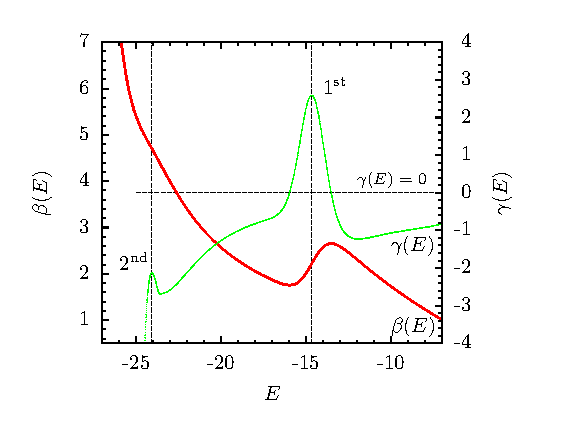
\includegraphics[width = 0.7\textwidth]{chapter2Figs/MicroAnalysisExample.eps}
\caption{\label{fig:Fig_1}%
Microcanonical inflection-point analysis of the inverse microcanonical temperature $\beta(E)$. The prominent back-bending region in $\beta(E)$, together with the positive-valued peak in its energy derivative $\gamma(E)$ at $E \approx -15$, indicates a \textit{first-order} transition. The negative-valued peak at $E\approx -24$ corresponds to a \textit{second-order} transition.}
\end{figure}
%

In analogy to the principle of minimal sensitivity~\cite{Stevenson}, structural transitions between pseudophases occur when $\beta (E)$, or one of its energy
derivatives, responds least sensitively to variations in energy. In particular, \textit{first-order} transitions are associated with inflection points in $\beta (E)$ that have a positive slope, accompanied by positive-valued peaks in the energy derivative $\gamma(E)=d\beta(E)/dE$. Similarly, a \textit{second-order} transition occurs when $\beta(E)$ exhibits an inflection point with a negative slope and $\gamma(E)$ attains a negative-valued peak. Examples of microcanonical \textit{first-} and \textit{second-order} transition signals are shown in Fig.~\ref{fig:Fig_1}. The formalism can be naturally extended to higher-order transitions. Inflection point in the $(2\mathrm{n})$th-derivative of entropy, accompanied by a positive-valued valley in the $(2\mathrm{n}+1)$th-derivative, indicates a $(2\mathrm{n}+1)$th-order transition. Similarly, a $(2\mathrm{n})$th-order transition is marked by an inflection point in the $(2\mathrm{n}-1)$th-derivative of entropy and a negative-valued peak in the $(2\mathrm{n})$th-order derivative.

%
\begin{figure}
\center
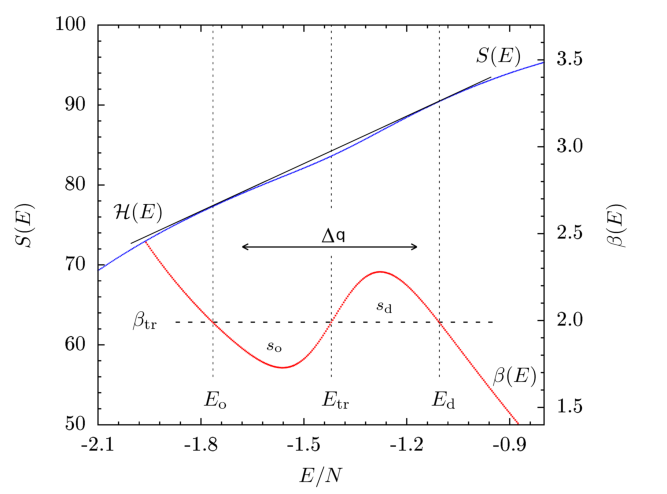
\includegraphics[width = 0.7\textwidth]{chapter2Figs/maxwellConstruct.pdf}
\caption{\label{fig:Fig_2}%
The convex region of the microcanonical entropy $S(E)$ and the back-bending of the microcanonical inverse temperature $\beta(E)$ are prominent indicators of \textit{first-order} transitions. The slope of the double-tangent Gibbs hull $\mathcal{H}(E)$ defines the transition temperature $\beta_{\mathrm{tr}}$. The Maxwell construction, defined by equal areas of $s_{\mathrm{o}}$ and $s_{\mathrm{d}}$, is itself positioned at $\beta_{\mathrm{tr}}$. The transition energy $E_{\mathrm{tr}}$ indicates the location of the largest separation between $\mathcal{H}(E)$ and $S(E)$, which signifies maximal entropic suppression of the transition states. The latent heat $\Delta Q$ corresponds to the width of the transition region between $E_{\mathrm{d}}$ and $E_{\mathrm{o}}$.}
\end{figure}
%
Alternatively, for \textit{first-order} transitions the transition temperature $\beta_{\mathrm{tr}}$ can be obtained by the means of the Maxwell construction, which was originally introduced to repair the unphysical back-bending in the pressure versus volume phase diagram for the van der Waals gas. However, in mesoscopic systems, finite-size effects lead to entropic suppression of the transition states, which is manifested in the backbending of $\beta(E)$ and the convex intruder in $S(E)$.Figure \ref{fig:Fig_2} shows an example of a Maxwell construction. Its position is determined by the equality of the areas $s_{\mathrm{o}}$ and $s_{\mathrm{d}}$. Often referred to as \textit{surface entropies}, $s_{\mathrm{o}}$ and $s_{\mathrm{d}}$ are defined in terms of the integrals
\begin{eqnarray}
\label{eq:surfaceEntr}
s_{\mathrm{o}} &=& \int_{E_{\mathrm{o}}}^{E_{\mathrm{tr}}} dE \:\: (\beta_{\mathrm{tr}}-\beta(E)), \\
s_{\mathrm{d}} &=& \int_{E_{\mathrm{tr}}}^{E_{\mathrm{d}}} dE \:\: (\beta(E)-\beta_{\mathrm{tr}}).
\end{eqnarray}
There are three intersections between the Maxwell line and the inverse temperature at energies $E_{\mathrm{o}}$, $E_{\mathrm{tr}}$, and $E_{\mathrm{d}}$. The separation between the boundary energies of the ordered pseudophase $E_{\mathrm{o}}$ and the disordered pseudophase $E_{\mathrm{d}}$, corresponds to the latent heat $\Delta Q = E_{\mathrm{d}} - E_{\mathrm{o}}$. The transition energy $E_{\mathrm{tr}}$ indicates the location where the intermediate states experience maximal entropic suppression.

The slope of the double-tangent Gibbs construction, also shown in Figure \ref{fig:Fig_2}, provides yet another definition of $\beta_{\mathrm{tr}}$. As a function of energy, the Gibbs hull is defined as
\begin{equation}
\mathcal{H}(E) = S(E_{\mathrm{o}}) + \beta_{\mathrm{tr}}[E-E_{\mathrm{o}}],
\end{equation}
where $\beta_{\mathrm{tr}}$ can be expressed in terms of the energy and entropy differences between the ordered and disordered pseudophases as
\begin{equation}
\beta_{\mathrm{tr}} = \frac{S_{\mathrm{d}}-S_{\mathrm{o}}}{E_{\mathrm{d}}-E_{\mathrm{o}}} = \frac{\Delta S}{\Delta Q}.
\end{equation}
With the exception of composite multi-step transitions, characterized by additional oscillations in the back-bending region of $\beta(E)$, the transition temperatures obtained by the means of the Maxwell and Gibbs constructions are identical.

The formalism of the microcanonical inflection-point analysis makes no reference to the thermodynamic limit. In fact, it is equally suitable for analysis of macroscopic and mesoscopic systems alike. This is in stark contrast to the more traditional canonical analysis which is defined under the assumption of the thermodynamic limit and has to be modified for the treatment of finite systems.

 
 
\section{The canonical ensemble}
\label{sec:canonicalEnsemble}
The canonical ensemble describes the behavior of a closed system in thermal equilibrium with a large external heat bath at a fixed temperature $T$. In analogy to the density of states in the microcanonical ensemble, the partition function $Z(T)$ contains all the essential information about the thermodynamic properties of the system under consideration. It can be defined directly as a Laplace transform\footnote{Here we assume that the system under investigation has discrete energy levels, which is always true in the context of computational studies. In the case of a continuous energy spectrum, the discrete sum is replaced by the integral $Z(T) = \int dE \:\:  g(E) e^{-\frac{E}{k_{\mathrm{B}}T}}$.} of the microcanical density of states $g(E)$
\begin{equation}
Z(T) = \sum g(E) e^{-\frac{E}{k_{\mathrm{B}}T}},
\end{equation}
where $T$ is the canonical heat bath temperature and $k_{\mathrm{B}}$ is the Boltzmann constant. While the condition of thermal equilibrium prohibits any net average energy transfer between the system and the heat bath, the system can gain or loose energy through constant fluctuations and dissipations. This leads to the well known temperature dependent Boltzmann distribution, where the probability for a given microstate $\mu$ is given by 
\begin{equation}
p(\mu) = \frac{1}{Z(T)}e^{-\frac{\mathcal{H}(\mu)}{k_{\mathrm{B}}T}},
\end{equation}
and $\mathcal{H}$ is the Hamiltonian of the system. The appropriate thermodynamic potential in the canonical ensemble is the Helmholtz free energy
\begin{equation}
F(T) = -k_{\mathrm{B}}T \: \mathrm{ln}\, Z(T).
\end{equation}
This quantity represents the energy available to perform work and can be used to obtain all other thermodynamic quantities by differentiation. The temperature derivative of the free energy defines the canonical entropy
\begin{equation}
S(T) = -\frac{\partial}{\partial T}F(T)\bigg|_{N,V},
\end{equation} 
which measures the amount of disorder in the system.
The internal energy $U$ is defined as a sum over all microstate energies weighted by the Boltzmann distribution  
\begin{equation}
U(T) = \frac{\sum_{\mu} \mathcal{H}(\mu)e^{-\frac{\mathcal{H}(\mu)}{k_{\mathrm{B}}T}}}{Z(T)} =  \frac{\sum_{E} E \, g(E) e^{-\frac{E}{k_{\mathrm{B}}T}}}{Z(T)}
\end{equation}
and represents the average energy of the system. Alternatively, the internal energy can be obtained by differentiating the free energy
\begin{equation}
U(T) = k_{\mathrm{B}}T^{2}\frac{\partial}{\partial T} \mathrm{ln} Z(T)\bigg|_{N,V}
= -T^{2}\frac{\partial}{\partial T}\left(\frac{F}{T}\right)\bigg|_{N,V}.
\end{equation}
The amount of energy needed to increase the temperature of the system by one unit is given by the specific heat 
$C_{V}$, defined as a temperature derivative of the internal energy
\begin{equation}\label{eq:22}
C_{V}(T) = \frac{\partial}{dT}U(T)\bigg|_{N,V} = -T\frac{\partial^{2}}{\partial T^{2}}F(T)\bigg|_{N,V},
\end{equation}
or differentiating the third term in equation 2.20 we get
\begin{eqnarray}
C_{V}(T) &=&  \frac{\partial}{dT}\frac{\sum_{E} E \, g(E) e^{-\frac{E}{k_{\mathrm{B}}T}}}{Z(T)} = -\frac{1}{k_{\mathrm{B}}T^2}\frac{\partial}{\partial \beta}\frac{\sum_{E} E \, g(E) e^{-\beta E}}{\sum_{E}g(E) e^{-\beta E}} \nonumber \\
&=& \frac{1}{k_{\mathrm{B}}T^2} \left[\left(\frac{\sum_{E} E^{2} \, g(E)  e^{-\beta E}}{Z(T)}\right) - \left(\frac{\sum_{E} E \, g(E)  e^{-\beta E}}{Z(T)}\right)^{2}\right] \nonumber \\
&=& \frac{1}{k_{\mathrm{B}}T^2}\left(\left<E^{2}\right> - \left<E\right>^{2}\right),
\end{eqnarray}
where the last expression corresponds to the variance of the Boltzmann distribution. This result is of a profound physical importance, establishing the connection between the macroscopic response quantity $C_{V}$, and microscopic fluctuations.

\subsection{Canonical analysis of phase transitions}
Sudden dramatic changes in macroscopic properties, as a response to small variations of an external control parameter, indicate that the system under investigation is undergoing a phase transition. Here we consider temperature-driven transitions and describe a classification scheme similar to Ehrenfest's.

In the thermodynamic limit, it is generally possible to identify some property of the system which is non-zero in the ordered phase and zero in the disordered phase, i.e. the order parameter. A standard example is the magnetization $m$ in a ferromagnetic system, where $m = 1$ in the ordered ferromagnetic phase and $m = 0$ in the disordered paramagnetic phase. The derivative of the order parameter with respect to its conjugate variable defines a response quantity\footnote{In the case of the magnetization $m$, the appropriate conjugate thermodynamic variable is the external field $H$, and the corresponding response quantity is the magnetic susceptibility $\chi$.} which is discontinuous at the transition point. Order parameters also play a central role in the formulation of the Landau theory, where they serve as a basis for the expansion of the free energy around the transition point. 

\begin{figure}
\center
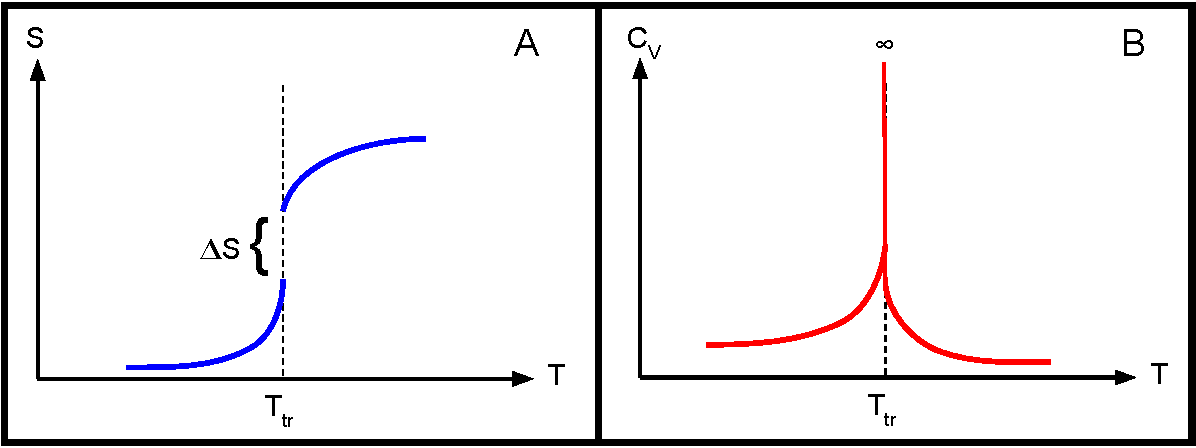
\includegraphics[width = 0.8\textwidth]{chapter2Figs/CanonicalFirstOrder.pdf}
\caption{\label{fig:Fig_3}% 
(Aa) The jump discontinuity in the canonical entropy $S$, and (b) the delta peak in the specific heat $C_{V}$, are characteristic of a first order phase transition.}
\end{figure} 

\begin{figure}
\center
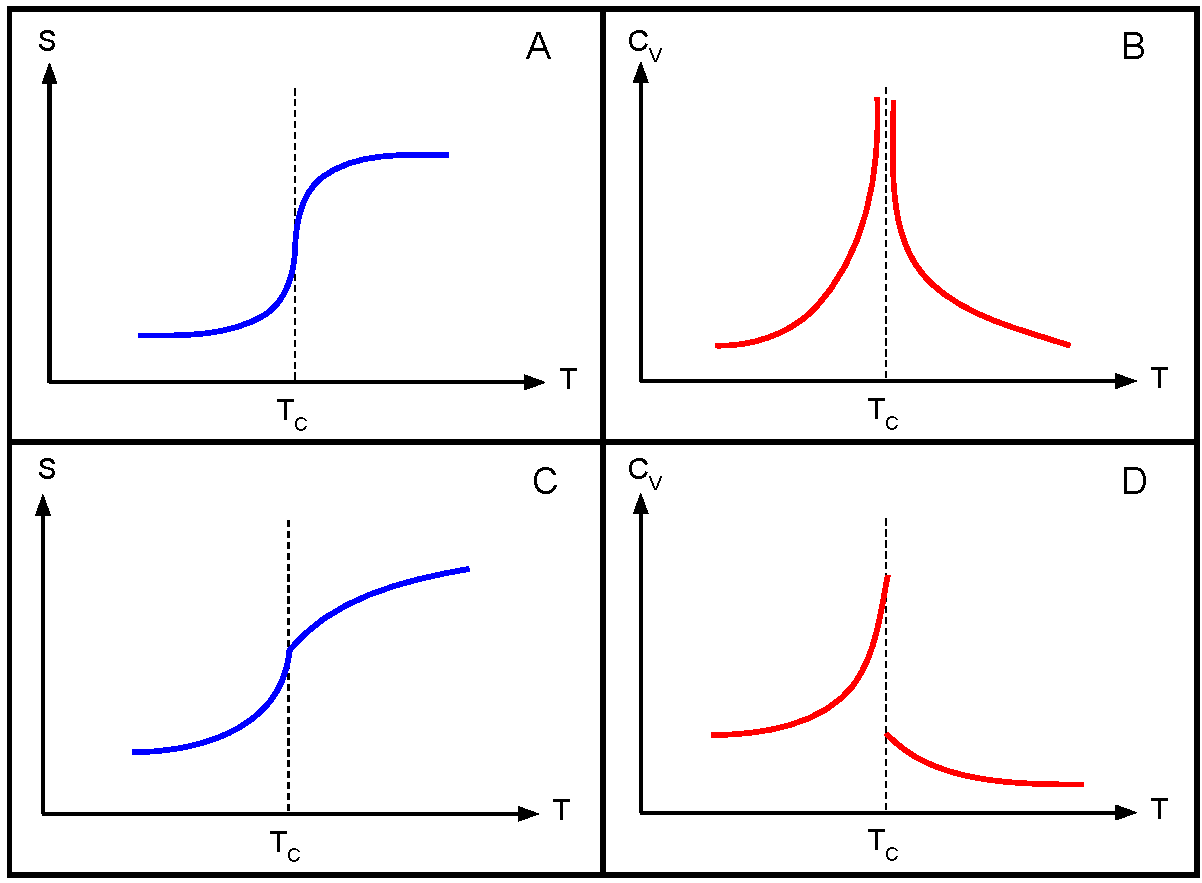
\includegraphics[width = 0.8\textwidth]{chapter2Figs/CanonicalSecondOrder.pdf}
\caption{\label{fig:Fig_4}% 
Second order transitions are characterized by discontinuities in response quantities, such as the specific heat. (a,b) In the case of a \textbf{critical} second order transition, the entropy $S$ attains an infinite slope at $T_{c}$ accompanied by a divergence in the specific heat $C_{V}$. (c,d) So called \textit{lambda} transitions are characterized by a jump discontinuity in $C_{V}$ and a cusp singularity in entropy.}
\end{figure}

First order transitions are characterized by a jump discontinuity in the entropy, also expressible as the negative of the first temperature derivative of the free energy. This results in the coexistence of two distinct phases\footnote{As a familiar example, consider the coexistence of gas bubbles and liquid at the boiling point of water.} at the transition temperature, whose energetic separation corresponds to the latent heat
\begin{equation}
\Delta Q = T_{\mathrm{trans}}\,\Delta S,
\end{equation}
where $\Delta S$ is the height of the discontinuity. The specific heat $C_{V}$ has a delta peak at the transition temperature, as shown in Fig. \ref{fig:Fig_3}.

Second order transitions do not posses discontinuities in entropy, and for that reason are often called \textit{continuous} transitions. Instead, discontinuities are found in the second derivative of the free energy with respect to temperature. It is customary to make use of the relationship shown in Eq.\,\,\ref{eq:22}, and consider the specific heat $C_{V}$ which also has the same discontinuities.
In the vicinity of the transition point $T_{c}$, the specific heat exhibits a power law behavior $C_{V}(\tau) \propto \left| \tau \right|^{-\alpha}$, where $\tau = \left(T-T_{c}\right)/T_{c}$ and $\alpha$ is the associated critical exponent. Examples of common types of discontinuities of $C_{V}$ are shown in Fig. \ref{fig:Fig_4}. Other important quantities such as the magnetic susceptibility $\chi$ and the correlation length $\xi$ also exhibit a power law behavior near the transition point, governed by the critical exponents $\gamma$ and $\nu$ respectively.

\subsubsection{Canonical analysis in mesoscopic systems} 
The description of phase transitions in the terms of discontinuities and divergences is valid only in the thermodynamic limit. In situations where the thermodynamic behavior of a system is affected by finite size effects, this idealized description no longer applies. Nevertheless, the numerous examples of abrupt changes of macroscopic properties in finite systems necessitate the generalization of the theory. In order to avoid possible confusion, we shall refer to significant conformational changes in finite systems as \textit{pseudophase transitions}. Similarly, sets of macrostates with sufficiently similar macroscopic properties will be denoted \textit{pseudophases}.

In the generalized formalism, peaks in the specific heat and other response quantities indicate regions of increased thermodynamic activity, i.e. pseudophase transitions. The order of the transition is determined from the shape of the canonical energy distribution in the transition region. Bimodal distributions reveal the coexistence of two pseudophases and indicate a first-order transition. The associated latent heat of the transition is given by the energetic separation of the two peaks in the distribution. Second-order transitions correspond to unimodal energy distributions. The power law behavior of response quantities contains significant finite-size corrections and in some cases is altogether not applicable. An example of canonical analysis, applied to first- and second-order pseudophase transitions, is illustrated in Fig. \ref{fig:Fig_5}. 

\begin{figure}
\center
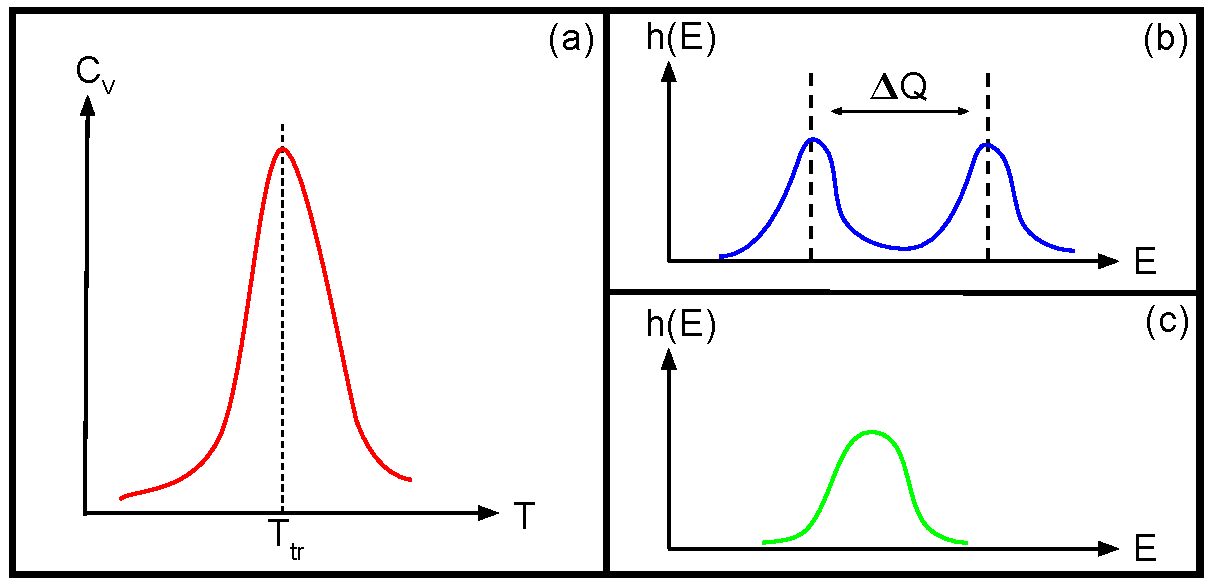
\includegraphics[width = 0.8\textwidth]{chapter2Figs/CanonicalAnalysisSample.pdf}
\caption{\label{fig:Fig_5}% 
(a) The peak in the specific heat $C_{V}$ indicates a region of heightened thermodynamic activity. (b) The two peaks in the bimodal canonical energy distribution correspond to the ordered and disordered pseudophases, energetically separated by the latent heat $\Delta Q$. Pseudophase coexistence and latent heat are reliable indicators of a first-order pseudophase transition. (c) Second-order transitions are marked by wide unimodal energy distributions at the transition point.}
\end{figure}

It should be mentioned that second-order pseudophase transitions do not always produce peaks in the specific heat. In general, it is necessary to investigate the behavior of several response quantities in order to obtain an accurate picture of the transition properties of the system under investigation. However, due to finite size effects, the signals obtained from different quantities will in general not coincide at a single transition temperature. This fact further fortifies the argument that the microcanonical inflection-point analysis\footnote{Introduced in Sec. \ref{subsec: micro_analysis}}, which defines a unique transition temperature in mesoscopic and macroscopic systems alike, is the preferred formalism for the analysis of finite systems.

\section{Alternative definitions of the density of states}
In section \ref{sec:mic_ensemble} we have defined the microcanonical density of states $g(E)$ as an integral over the surface of constant energy in the $6N$-dimensional phase space. We have argued that $g(E)$ contains all the essential information about the thermodynamic properties of the system under consideration, and introduced the formalism of the microcanonical inflection-point analysis which uses the logarithm of $g(E)$ as its starting point. In section \ref{sec:canonicalEnsemble} we have shown that the canonical partition function $Z(T)$ can be obtained by performing a Laplace transform of $g(E)$. Clearly, the microcanonical density of states plays a fundamental role in equilibrium statistical mechanics, and as such needs to be carefully defined. 

Two different definitions of the density of states arise from the ambiguity of the exact meaning of the microcanonical ensemble in computational studies. The density of states can be defined in the context of the conformational microcanonical ensemble $(N,V,E_{p})$ as a function of the potential energy only
\begin{equation}
g_{c}(E_{p}) = \int \mathcal{DQ} \:\: \delta(E_{p} - \mathcal{H}(\mathcal{Q}))
\end{equation}
This definition is commonly used in Monte Carlo simulations of magnetic systems where the kinetic energy contributions have little physical significance and the sampling can be restricted to the conformational space only. However, in systems where the transfer between potential and kinetic energy has important physical interpretation, the sampling of the full phase space becomes necessary. The standard definition of the microcanonical ensemble $(N,V,E)$ is appropriate and the measured density of states is a function of the total system energy, which can be written as the sum of the potential and kinetic energies
\begin{equation}
E = E_{p} + E_{k}.
\end{equation}
In order to distinguish between the two definitions, we shall use the symbol $\Gamma(E)$ to represent the full density of states. The connection between the conformational density of states and $\Gamma(E)$ is expressed as a convolution
\begin{equation}
\label{eq:TotalDOS}
\Gamma(E) = \int dE_{k} \: g_{c}(E - E_{k})g_{k}(E_{k}),
\end{equation}
where 
\begin{equation}
g_{k}(E_{k}) = \int \mathcal{DP} \:\: \delta(E_{k} - \mathcal{H}(\mathcal{P}))
\end{equation}
is the kinetic density of states obtained by integrating over the momentum space.

We shall now turn our attention to the consequence of choosing either the conformational or the full density of states as the starting point of a systematic analysis of the thermodynamic properties of the system under consideration. For this purpose, we will discuss the impact of including the momentum degrees of freedom, on the results of both the canonical and microcanonical analysis. As an illustration, we will provide results from Monte Carlo simulations of two short flexible homopolymers.

\subsection{Consequences for canonical analysis}
The canonical partition function $Z(T)$ and the microcanonical density of states are connected via a Laplace transform. We begin with the full density of states $\Gamma(E)$ and using the definition from Eq. \ref{eq:22} write
\begin{equation}
\label{eq:Laplace}
Z(T) = \mathcal{L}\left\lbrace\Gamma(E)\right\rbrace = \mathcal{L}\{g_{c} \ast g_{k} \} = \mathcal{L}\{g_{c}\} \mathcal{L}\{g_{k}\},
\end{equation}
where the last step follows from the convolution theorem. The partition function of the system can therefore be written as a product of two independent partition functions
\begin{equation}
Z(T) = Z_{c}(T)Z_{k}(T),
\end{equation}
which depend on the potential and kinetic energies respectively. It follows that the average ensemble energy can be expressed as the sum of the average potential and kinetic energies
\begin{eqnarray}
U(T)  &=& k_{\mathrm{B}}T^{2}\frac{\partial}{\partial T} \mathrm{ln} Z\bigg|_{N,V} \nonumber \\
	 &=& k_{\mathrm{B}}T^{2}\frac{\partial}{\partial T} \mathrm{ln} Z_{c} \bigg|_{N,V}	 + k_{\mathrm{B}}T^{2}\frac{\partial}{\partial T} \mathrm{ln} Z_{k} \bigg|_{N,V}	 \nonumber \\
	 &=& \langle E_{c} \rangle + \langle E _{k}\rangle.  
\end{eqnarray}
With the exception of systems with rigid constraints, the average kinetic energy is given by the equipartition theorem 
\begin{equation}
 \langle E _{k}\rangle = \frac{3Nk_{\mathrm{B}}T}{2},
\end{equation}
where $N$ is the number of particles in the system. It follows that the specific heat $C_{\mathrm{V}}$ obtains only a trivial additive constant from the kinetic energy term
\begin{eqnarray}
C_{\mathrm{V}}(T) &=& \frac{\partial}{\partial T} U(T)\bigg|_{N,V} \nonumber \\
				 &=& \frac{\partial}{\partial T} \langle E_{c} \rangle\bigg|_{N,V} + \frac{\partial}{\partial T}\frac{3Nk_{\mathrm{B}}T}{2} \nonumber \\
				 &=& C_{\mathrm{V},\mathrm{conf.}} + \frac{3Nk_{\mathrm{B}}}{2}.
\end{eqnarray}

\begin{figure}
\center
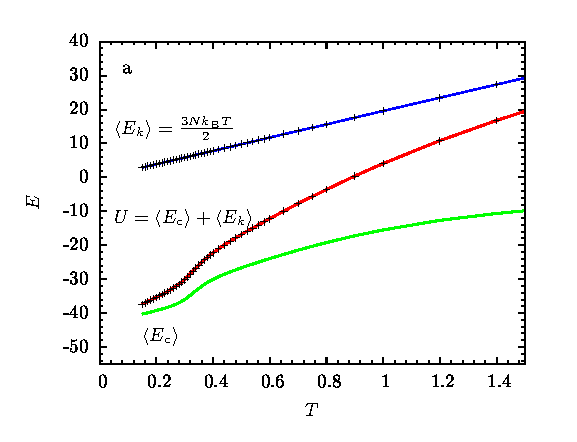
\includegraphics[width = 0.49\textwidth]{chapter2Figs/N13Energy.eps}
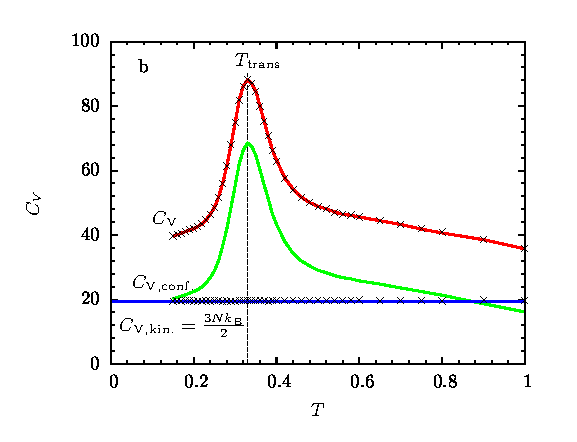
\includegraphics[width = 0.49\textwidth]{chapter2Figs/N13Spec.eps}
\caption{\label{fig:Fig_6}% 
Results of a Monte Carlo simulation of a short flexible homopolymer of length $N=13$. The average kinetic energy $\langle E _{k}\rangle$ and the kinetic contributions $C_{\mathrm{V,kin.}}$ towards the specific heat are plotted as points on top of their respective theoretical curves (blue). The average potential energy $\langle E_{c} \rangle$ and the configurational specific heat $C_{\mathrm{V},\mathrm{conf.}}$ (green) were obtained by sampling of the configurational space. Sampling of the full phase space was performed to obtain the total average energy $U$ and the combined specific heat $C_{\mathrm{V}}$ (red). As expected, the combined specific heat is identical to $C_{\mathrm{V},\mathrm{conf.}}$, except for a trivial additive constant.}
\end{figure}

In conclusion, the locations and shapes of pseudophase transition signals are unaffected by the inclusion of the momentum space into a sampling scheme. To substantiate this assertion, we present the results of a Monte Carlo study of a short flexible homopolymer in Fig. \ref{fig:Fig_6}. The average kinetic energy $\langle E _{k}\rangle$ and the kinetic contributions $C_{\mathrm{V,kin.}}$ towards the specific heat are plotted as points on top of their respective theoretical curves (blue), showing good agreement with the predicted values. The average potential energy $\langle E_{c} \rangle$ and the configurational specific heat $C_{\mathrm{V},\mathrm{conf.}}$ (green) were obtained by sampling restricted to the configurational space only. Sampling of both the momentum and configurational space was performed to obtain the total average energy $U$ and the combined specific heat $C_{\mathrm{V}}$ (red). As expected, the combined specific heat is identical to $C_{\mathrm{V},\mathrm{conf.}}$, except for a trivial additive constant. The estimate of the transition temperature is independent of the choice of either definition of the density of states. 
\newpage 

\subsection{Consequences for microcanonical analysis}
The application of the Laplace transform to the total density of states $\Gamma (E)$ conveniently allowed us to disentangle the convolution in Eq. \ref{eq:TotalDOS} \, into separate kinetic and conformational contributions [Eq. \ref{eq:Laplace}]. Unfortunately, in the microcanonical ensemble no such simplification is readily available. Let us however consider a class of physical systems whose momenta and positional degrees of freedom are independent. Explicit integration over the momentum space yields 
\begin{equation}
g_{k}(E_{k}) = \int \mathcal{DP} \:\: \delta(E_{k} - \mathcal{H}(\mathcal{P})) 
			 = E_{k}^{\frac{3N-2}{2}}.
\end{equation}
Combining the result with Eq. \ref{eq:TotalDOS} \, we get
\begin{equation}
\Gamma(E) = \int dE_{k} \: g_{c}(E - E_{k})E_{k}^{\frac{3N-2}{2}}.
\end{equation}
Next, taking a derivative with respect to the total energy $E$ and dividing both sides by $\Gamma(E)$ we obtain two equivalent expressions for the microcanonical inverse temperature 
\begin{eqnarray}
\beta(E) &=& \int dE_{k} \:\frac{3N-2}{2E_{k}} \:\left[\frac{g_{c}(E - E_{k})E_{k}^{\frac{3N-2}{2}}}{\Gamma (E)}\right]
\label{eq:beta1}  \\
		&=& \int dE_{p} \: \beta_{c}(E_{p})\: \left[ \frac{g_{c}(E_{p})(E- E_{p})^{\frac{3N-2}{2}}}{\Gamma (E)} \right]
\label{eq:beta2}.  
\end{eqnarray}
Recognizing the two terms enclosed in square brackets as the microcanonical probability densities for the kinetic and potential energies,
\newpage
\noindent
we can rewrite equations \ref{eq:beta1} and \ref{eq:beta2} as
\begin{equation}
\label{eq:beta3}
\beta(E) = \int dE_{k} \:\frac{3N-2}{2E_{k}} \: \rho(E_{k}|E) = \frac{3N-2}{2}\left\langle \frac{1}{E_{k}}  \right\rangle,
\end{equation}
and 
\begin{equation}
\label{eq:beta4}
\beta(E) = \int dE_{p} \: \beta_{c}(E_{p})\: \rho(E_{p}|E) = \left\langle \beta_{c} \right\rangle.
\end{equation}
The microcanonical inverse temperature, obtained by the differentiation of the total density of states, can therefore be interpreted as an average of the conformational and kinetic anologs weighted by their respective microcanonical probability distributions.

When the number of particles in the system is large, the probability densities $\rho(E_{k}|E)$ and $\rho(E_{p}|E)$ are expected to be sharply peaked. We can therefore apply the saddle point approximation to the integrals in equations [\ref{eq:beta3}, \ref{eq:beta4}] and obtain the following first order approximations for the inverse temperature
\begin{equation}
\label{eq:approx1}
\beta(E) \approx \beta_{c}(\bar{E}_{p}),
\end{equation}
and
\begin{equation}
\label{eq:approx2}
\beta(E) \approx \frac{3N-2}{2}\left(\frac{1}{E-\bar{E}_{p}}\right), 
\end{equation}
where $\bar{E}_{p}$ is the most probable potential energy corresponding to the peak of the distributions. The two expressions suggest that it is possible to reconstruct  $\beta(E)$ from the conformational inverse temperature $\beta_{c}$, and that the two quantities contain essentially the same information. We test the validity of this hypothesis by comparing the microcanonical results of Monte Carlo simulations in the conformational and the full phase space, as applied to a flexible elastic $55-$mer.

The kinetic entropy in Fig. \ref{fig:Fig_7} is a strictly concave function and the application of the inflection-point analysis to the corresponding inverse temperature $\beta_{k}$ reveals no transition signals. The conformational inverse temperature clearly differs from $\beta(E)$, however both indicate a first-order pseudophase transition at virtually the same temperature. In Fig. \ref{fig:Fig_8} we show the comparison between the true $\beta(E)$ and the reconstruction obtained from the conformational inverse temperature according to equations \ref{eq:approx1} and \ref{eq:approx2}. It is evident that the approximation is valid, except in the back-bending region of the first-order transition due to the bimodality of the probability densities $\rho(E_{k}|E)$ and $\rho(E_{p}|E)$. This will lead to differences in the estimated free energy barrier associated with the transition.


\begin{figure}
\center
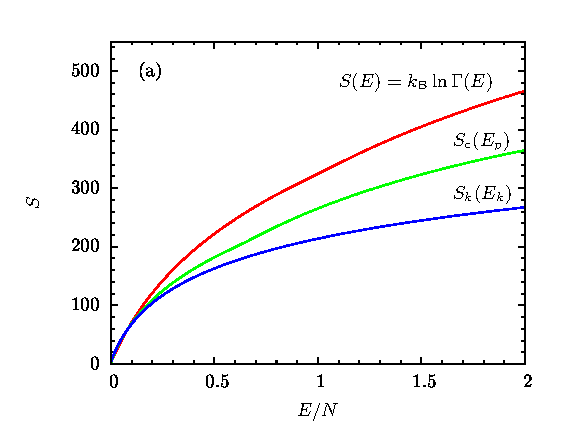
\includegraphics[width = 0.49\textwidth]{chapter2Figs/N55Entropy.eps}
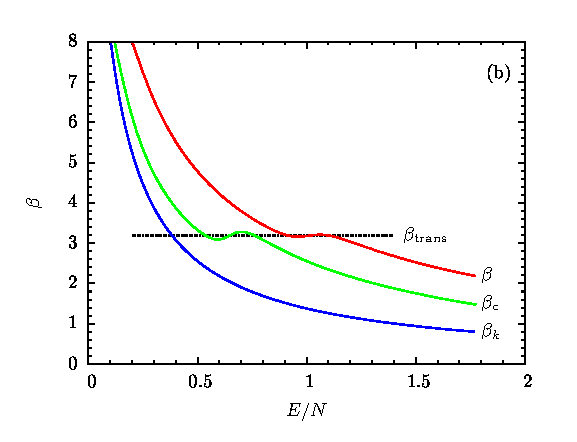
\includegraphics[width = 0.49\textwidth]{chapter2Figs/N55Beta.eps}
\caption{\label{fig:Fig_7}% 
Comparison of microcanonical results from a Monte Carlo simulation of a flexible homopolymer of length $N=55$.(a) The combined $S$, conformational $S_{c}$, and kinetic $S_{k}$ entropy curves. (b) The kinetic inverse temperature $\beta_{k}$ is a strictly convex function and the application of the inflection-point analysis reveals no transition signals. The conformational inverse temperature $\beta_{c}$ clearly differs from $\beta(E)$, however both indicate a first-order pseudophase transition at virtually the same temperature. }
\end{figure}

\begin{figure}
\center
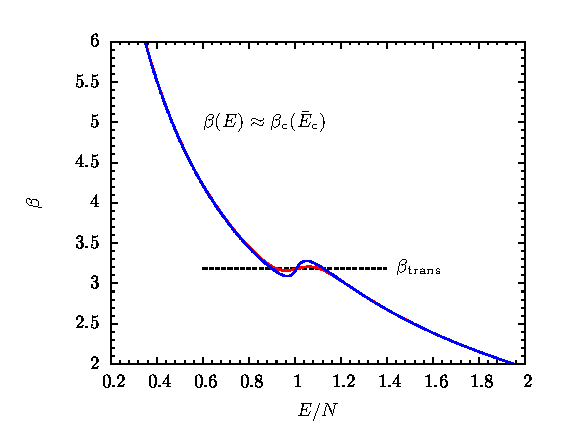
\includegraphics[width = 0.7\textwidth]{chapter2Figs/N55BetaComp.eps}
\caption{\label{fig:Fig_8}% 
Comparison of the inverse microcanonical temperature $\beta(E)$ (red) and the conformational inverse temperature $\beta_{c}(\bar{E}_{p})$ (blue) evaluated at the most probable potential energy $\bar{E}_{p}$. The approximation introduced in equations \ref{eq:approx1} and \ref{eq:approx2} holds except in the back-bending region of the first-order pseudophase transition. The inverse transition temperature $\beta_{\mathrm{trans}}$ obtained from the two quantities is virtually identical, however the estimated free energy barrier is higher for $\beta_{c}$.}
\end{figure}












 


\chapter{Computational Methods}
\section{Markov chain Monte Carlo}
\subsection{Master equation and detailed balance}
\subsection{Metropolis sampling}
\section{Generalized ensemble Monte Carlo}
\subsection{Parallel tempering}
\subsection{Multiple Gaussian modified ensemble}
\subsection{Histogram reweighting methods}
\subsection{Multicanonical sampling}
\section{Simple Monte Carlo updates}

\chapter{Coarse-grained Homopolymer Model}
\section{Flexible elastic homopolymer}
\section{Interacting homopolymers}

\chapter{Confinement Effects on Structural Transitions in Flexible Homopolymers}
\section{Introduction}
\section{Canonical analysis}
\section{Inflection-point analysis}
\section{Hyper-phase diagrams}

\chapter{Impact of Bonded Interactions on the Ground-State Geometries of Flexible Homopolymers}
\section{Structural order parameters}
\section{15-mer}
\section{55-mer}

\chapter{Aggregation of Flexible Elastic Homopolymers}
\section{Introduction}
\section{Microcanonical analysis}
\subsection{Subphases and subphase transitions}
\subsection{Missing subphases and translational entropy}
\subsection{Density effects on the latent heat}

\chapter{Summary and Outlook}










\begin{figure}
\centerline{[ You could put a picture here. ]}
\caption{Example of a figure.}
\end{figure}

\begin{table}
\caption{Example of a table.}
\centerline{[The contents of the table would go here.]}
\end{table}



%~~~~~~~~~~~~~~~~ Reference ~~~~~~~~~~~~~~~~~~%
\addcontentsline{toc}{chapter}{Bibliography}
\begin{thebibliography}{99}
        %%%%%%%%%%% CHAPTER 2 %%%%%%%%%%%%%%%%%%
\bibitem{Bachmann2014}
M.~Bachmann, \emph{Thermodynamics and Statistical Mechanics of
Macromolecular Systems}, (Cambridge University Press, Cambridge,
2014).
%
\bibitem{Rugh2001}
H.~H.~Rugh , Phys.\ Rev.~E \textbf{64},
055101 (2001).

%%%%%%%%%%% Microcanonical Ensemble %%%%%%%%%%%

\bibitem{Kardar2007}
M.~Kardar, \emph{Statistical Physics of Particles}, (Cambridge University Press, New York, 2007).
%
\bibitem{Pathria}
R.~K.~Pathria, and P.~D.~Beale, \emph{Statistical Mechanics}, (Elsevier, Oxford, 2011).
%
\bibitem{Sethna2006}
J.~P.~Sethna, \emph{Statistical Mechanics: Entropy, Order Parameters, and Complexity}, 
(Oxford University Press, New York, 2006).
%


%%%%%%%%%%% Microcanonical Analysis %%%%%%%%%%%%
\bibitem{Gross2001} 
D.~H.~E.~Gross, \emph{Microcanonical Thermodynamics}, (World Scientific, Singapore,  2001).
%
\bibitem{Stevenson}
P.~M.~Stevenson, Phys.\ Rev.~D \textbf{23}, 2916 (1981).
%
\bibitem{Schnabel2011}
S.~Schnabel, D.~T.\ Seaton, D.~P.\ Landau, and M.~Bachmann, Phys.\ Rev.~E
\textbf{84}, 011127 (2011). 
%


%%%%%%%%%%% Canonical Analysis %%%%%%%%%%%%%%%%

\bibitem{Landau2000}
D.~P.\ Landau, and K.~Binder, \emph{A Guide to Monte Carlo Simulations in Statistical Physics}, (Cambridge University Press, Cambridge, 2000).

%%%%%%%%%%% Definitions of Density of States %%%%%%%%%

\bibitem{Calvo1995}
F.~Calvo, and P.~Labastie,  Chem.\ Phys.\ Lett. \textbf{247}, 395 (1995).
%




\end{thebibliography}


\end{document}


